\documentclass{beamer}
\usetheme{default}
\usepackage{listings}
\usepackage{color}
\usepackage{hyperref}
\usepackage{polski}
\usepackage[polish]{babel}
\usepackage[utf8]{inputenc}
\usepackage{amssymb}


\title{Entropia i jej zastosowania}
\author{Andrzej Pragacz}

\begin{document}

\titlepage

\section{Podstawowe pojęcia}

\begin{frame}{Przestrzeń probabilistyczna (prawdopodobieństwo klasyczne)}
Tzw. przestrzeń probabilistyczna składa się z:
\begin{itemize}
  \item Zbioru $\Omega$, będącego skończonym zbiorem zdarzeń
  elementarnych $\omega$. Każde ze zdarzeń $\omega$ może wystąpić z jednakowym
  prawdopodobieństwem.
  \item Funkcji prawdopodobieństwa $P: 2^\Omega \to [0, 1]$ zdefiniowanej:
  $$
  P(A) = \frac{|A|}{|\Omega|}
  $$
  o własnościach:
  \begin{itemize}
    \item $P(\emptyset) = 0$
    \item $P(\Omega) = 1$
    \item $P(A \cup B) = P(A) + P(B)$ jeśli $A \cap B = \emptyset$
  \end{itemize}
\end{itemize}
\end{frame}

\begin{frame}{Zmienna losowa (prawdopodobieństwo klasyczne)}
\begin{itemize}
  \item Zmienna losowa $X$ to funkcja typu $\Omega \to S$, gdzie $S$ jest
  zbiorem elementów (najczęściej skończonym)
  \item Przykłady:
  \begin{itemize}
    \item $X$ jako liczba wyrzuconych oczek. Wówczas: $$P(X=1) = P(X=2) = \ldots = P(X=6) = \frac{1}{6}$$
    \item $X$ jako litera występująca z prawdopodobieństwem występowania
    w losowym tekście. Przykładowo:
    $$ P(X=E) = 0.1249, P(X=T) = 0.0928, P(X=A) = 0.0804 \ldots$$
  \end{itemize}
\end{itemize}
\end{frame}

\begin{frame}{Niezależność i prawdopodobieństwo warunkowe}
\begin{itemize}
  \item Zdarzenia $A$ i $B$ są niezależne, jeśli $P(A \cap B) = P(A) P(B)$
  \item Zmienne losowe $X_1$ i $Y_1$ są niezależne, jeśli dla każdych
  $T_1 \subseteq S_1$, $T_2 \subseteq S_2$ zachodzi:
  $P(X_1 \in T_1, X_2 \in T_2) = P(X_1 \in T_1) P(X_2 \in T_2)$
  \item Prawdopodobieństwo warunkowe względem zdarzenia $B$
  (przy założeniu, że $P(B) > 0$) definiujemy jako:
  $$
  P(A|B) = \frac{P(A \cap B)}{P(B)}
  $$
\end{itemize}
\end{frame}

\section{Entropia}

\begin{frame}{Gra w 20 pytań}
\begin{center}

\includegraphics[width=0.5\textwidth]{img/akinator.png}
\end{center}
\end{frame}


\begin{frame}{Gra w n pytań}
\begin{itemize}
  \item niech będzie dane 8 liczb $1, 2, \ldots, 8$. Każdą z nich można wylosować
  z jednakowym prawdopodobieństwem, co będzie reprezentowane
  przez zmienną losową $X$. ile pytań (tak/nie) średnio potrzeba żeby odgadnąć
  wylosowaną liczbę?
  \pause
  \item średnio: 3 pytań
  \item a co jeśli przyjmiemy że $P(X=1) = 1$ (pozostałe prawdopodobieństwa się zerują)?
  \pause
  \item 0 pytań!
\end{itemize}
\end{frame}

\begin{frame}{Gra w n pytań - drzewo decyzyjne}
\begin{center}
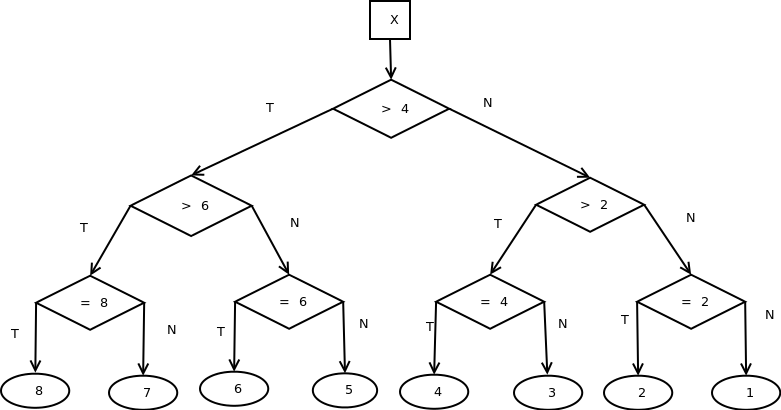
\includegraphics[width=0.9\textwidth]{img/decision_tree1.png}
\end{center}
Ścieżka od korzenia do liścia = lista pytań = kod binarny
\end{frame}


\begin{frame}{Gra w n pytań c.d.}

\begin{itemize}
  \item a co jeśli:
  $$
  P(1) = \frac{1}{2}, P(2) = \frac{1}{2^2}, \ldots, P(7) = P(8) = \frac{1}{2^7}
  $$
  \pause
  \item Przykładowe rozwiązanie:
  \begin{itemize}
    \item Pytamy czy $X=1$.
    \item Jeśli nie, to pytamy czy $X=2$.
    \item $\ldots$
    \item Jeśli nie, to pytamy czy $X=7$.
    \item Jeśli nie, to $X=8$.
  \end{itemize}
  \item Średnia liczba pytań:
  $$\frac{1}{2} + 2 \frac{1}{2^2} + 3 \frac{1}{2^3} + \ldots + 6 \frac{1}{2^6} +2 \cdot 7 \frac{1}{2^7} = 1.984375$$
  \item A co jeśli mamy ogólny rozkład? jaka jest dolna granica średniej liczby pytań?
\end{itemize}
\end{frame}


\begin{frame}{Entropia}
Niech $X$ będzie zmienną losową w zbiór $S = \{s_1, s_2, \ldots, s_n\}$
oraz $P(X=s_i) = p_i$. \textbf{Entropia} $X$ to:
$$
H_r(X) = \sum_{i=1}^{n} p_i \log_{r}{\frac{1}{p_i}} = - \sum_{i=1}^{n} p_i \log_{r}{p_i}
$$

Czasem $H_r(X)$ nazywa się również zawartością informacyjną bądź miarą niepewności.

Przyjmujemy, że $0 \log_r{0} = 0 \log_r{\frac{1}{0}} = 0$.

\end{frame}


\begin{frame}{Entropia c.d.}

Ograniczenie dolne i górne:
\begin{itemize}
  \item jeśli dla pewnego $p_i$ zachodzi $p_i = 1$ to $H_r(X) = 0$ (wartość minimalna)
  \item jeśli $p_1 = p_2 = \ldots = p_n$ to $H_r(X) = \log_r{n}$ (wartość maksymalna)
\end{itemize}

\end{frame}


\section{Zastosowania}

\subsection{Entropia jako dolne ograniczenie na liczbę pytań}


\begin{frame}{Entropia jako dolne ograniczenie na liczbę pytań}

Niech $l(s_i)$ będzie liczbą pytań (tak/nie) potrzebną żeby odgadnąć
dane $s_i \in S$ przy zadanej strategii $l$. Wówczas dla każdej
strategii $l$:

$$
H_2(X) \leq \sum_{i=1}^{n} p_i l(s_i)
$$

\end{frame}


\begin{frame}{Interludium}
\begin{center}
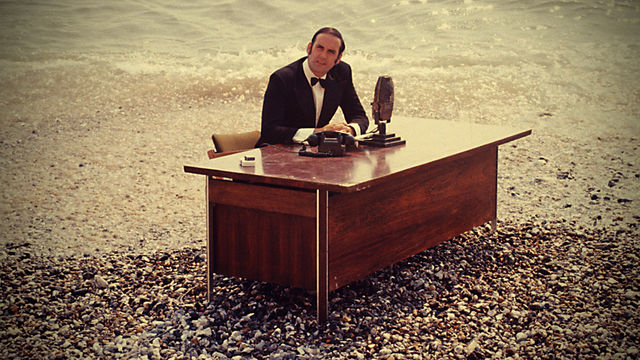
\includegraphics[width=0.9\textwidth]{img/cleese-at-ocean-desk.jpg}
\end{center}
\end{frame}

\begin{frame}{Nierówność Jensena}
Funkcję $f$ spełniającą nierówność:
$$
f\left(\frac{x + y}{2}\right) \leq \frac{f(x) + f(y)}{2}
$$
nazywamy funkcją \textbf{wypukłą}. Alternatywna definicja to $f'' \geq 0$.
\newline

Dla takich funkcji zachodzi \textbf{nierówność Jensena};
niech $\sum_{i=1}^{n} a_i = 1$, $a_i > 0$, wówczas:
$$
f\left(\sum_{i=1}^{n} a_i x_i\right) \leq \sum_{i=1}^{n} a_i f(x_i)
$$
(dowód przez indukcję)
\end{frame}

\begin{frame}{Złoty lemat}
Niech $\sum_{i=1}^{n} p_i = 1$, $p_i > 0$ oraz $\sum_{i=1}^{n} q_i \leq 1$, $q_i > 0$. Wówczas:

$$
\sum_{i=1}^{n} p_i \log{\frac{1}{p_i}} \leq \sum_{i=1}^{n} p_i \log{\frac{1}{q_i}}
$$

Dowód: oznaczając $f(x) = x \log{x}$ jako funkcję wypukłą korzystamy
z nierówności Jensena:

$$
P - L = \sum_{i=1}^{n} p_i \log{\frac{p_i}{q_i}}
= \sum_{i=1}^{n} q_i \left(\frac{p_i}{q_i}\right) \log{\frac{p_i}{q_i}}
$$
$$
\geq \left( \sum_{i=1}^n q_i \cdot \frac{p_i}{q_i} \right) \log{\left( \sum_{i=1}^n q_i \cdot \frac{p_i}{q_i} \right)}
= 0
$$

\end{frame}


\begin{frame}{Entropia jako dolne ograniczenie - dowód}

Dla dowolnej strategii zadawania pytań $l$ podstawiamy
$q_i = \frac{1}{2^{l(s_i)}}$ do złotego lematu i uzyskujemy nierówność

$$
H_2(X) \leq \sum_{i=1}^{n} p_i l(s_i)
$$

Warunek:

$$
\sum_{i=1}^n q_i = \sum_{i=1}^n \frac{1}{2^{l(s_i)}} \leq 1
$$
zachodzi i nazywa się \textbf{nierównością Krafta}.
\end{frame}


\subsection{Kryptografia}

\begin{frame}{Smutny fakt z kryptografii}
Niech $M$ będzie wiadomością, $K$ kluczem a $C$ wynikowym kryptogramem. Inaczej mówiąc:
$$
C = Enc(M, K), M = Dec(C, K)
$$
Jeśli potraktujemy $C, K, M$ jako zmienne losowe, to jeśli $C$ i $M$ są niezależne
to kryptosystem jest \textbf{idealnie bezpieczny}. Wówczas:
$$
H_2(K) \geq H_2(M)
$$
Inaczej mówiąc, klucz musi być conajmniej takiej długości co wiadomość.
\end{frame}


\subsection{Drzewa decyzyjne}

\begin{frame}{Budowanie drzew decyzyjnych}
\end{frame}


\subsection{Mechanika statystyczna i termodynamika}

\begin{frame}{Entropia a mechanika statystyczna i termodynamika}

System $X$ składa się z $W$ mikrostanów $x_i$ (konfiguracji położenie/pęd cząsteczek), gdzie stan
$x_i$ występuje z prawdopodobieństwem $p_i$. Entropię takiego systemu definiujemy
następująco:

$$
S = - k_B \sum_{i=1}^{W} p_i \ln{p_i}
$$

gdzie $k_B = 1.38065 \cdot 10^{-23} J/K$.
W praktyce często rozpatrujemy mikrostany o tych samych energiach i które mają
to samo prawdopodobieństwo występowania, więc wzór upraszcza sie do:

$$
S = k_B \ln{W}
$$

\end{frame}

\begin{frame}{Bibliografia}
\begin{itemize}
  \item Wstęp do teorii prawdopodobieństwa, J.Jakubowski, R. Sztencel
  \item \url{http://wazniak.mimuw.edu.pl/index.php?title=Teoria_informacji}
  \item \url{https://www.khanacademy.org/science/physics/thermodynamics}
  \item \url{http://norvig.com/mayzner.html}
\end{itemize}
\end{frame}


\end{document}
